\subsection{Introduction}
Avoid treating parameters as randome variables.
The notion of variation across repeated trials forms the basis for modelling
uncertainity.


\subsection{Hypothesis Testing}
A \emph{frequentist} statistics, probabilities represent the frequencies at which 
particular events happen.

\subsection{\emph{p-value}}
It is the heart of frequentist hypothesis testing, it tells us the \tB{probability of 
getting a particular test statistic $t$ as big as the one we have or bigger under the null
hypothesis} (that there is actually no effect).\\
By convention we usually conclude an effect is \emph{statistically significant} if the 
\emph{p-value} is less than a threshold $\alpha$.

\subsection{Confidence intervals}
When we fit a model to our data we look for the \emph{maximum of likelihood} parameters,
meaning the parameters that are most consistent with our data. 
For each parameter we will able to construct $95\%$ interval namely \tB{$95$ of the $100$ 
intervals generated will contain the true value of the parameter}.\\
If $H_{0}: \beta=0$ is true, the probability of getting a $95\%$ confidence interval that
does not include 0 is less than 0.05. In other words, if the $95\%$ confidence does not 
include 0, $p<0.05$.
\begin{figure}[H]
	\begin{center}
		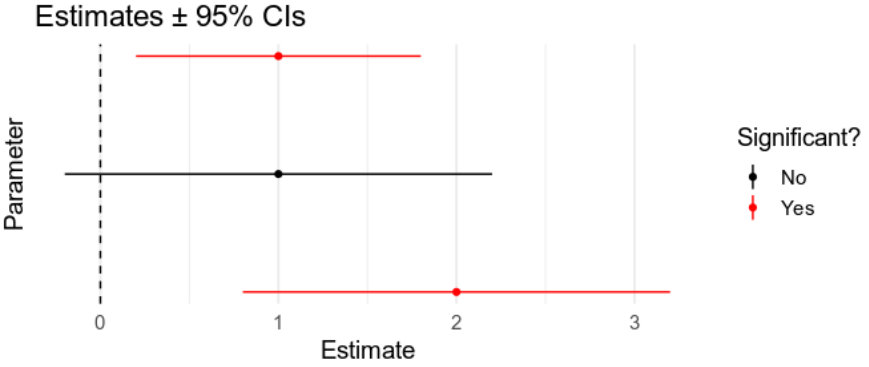
\includegraphics[width=\textwidth]{./chapters/2_statistics/04_frequentist_approach/4_images/1_estimates.png}
	\end{center}
	\caption{Confidence interval}
	\label{fig:2.4.1_estimates}
\end{figure}

\subsection{Multiple comparisons}
The more tests we run the more likely it is to we'll find at least one that is significant
even though the null hypothesis is true. We can then apply a Bonferroni correction.\\
Let's say we are running $k$ tests, we can either adjust: 
\begin{itemize}
	\item the threshold $\alpha_{adj} = \dfrac{\alpha}{k}$ OR
	\item the \emph{p-value} $p_{ajd} = k\times p$
\end{itemize}


